\section{Circuit Analysis with Diode}
Trong PSpice, một số bài tập trong bài có thể được mô phỏng để xác nhận kết quả. Mặc dù
nó không hoàn toàn giống các giá trị (ví dụ: điện áp và dòng điện), mô phỏng trong PSpice là một
công cụ để kiểm tra giải pháp của bạn. Một mạch mô phỏng ví dụ có diode và điện trở là
được miêu tả như sau:

Sinh viên được đề xuất phân tích mạch này bằng mô hình diode thực tế, với điện áp rơi khoảng 0,7V. Sau đó chạy mô phỏng trên PSpice để kiểm tra lại với
kết quả của bạn.

\begin{figure}[h]
    \centering
    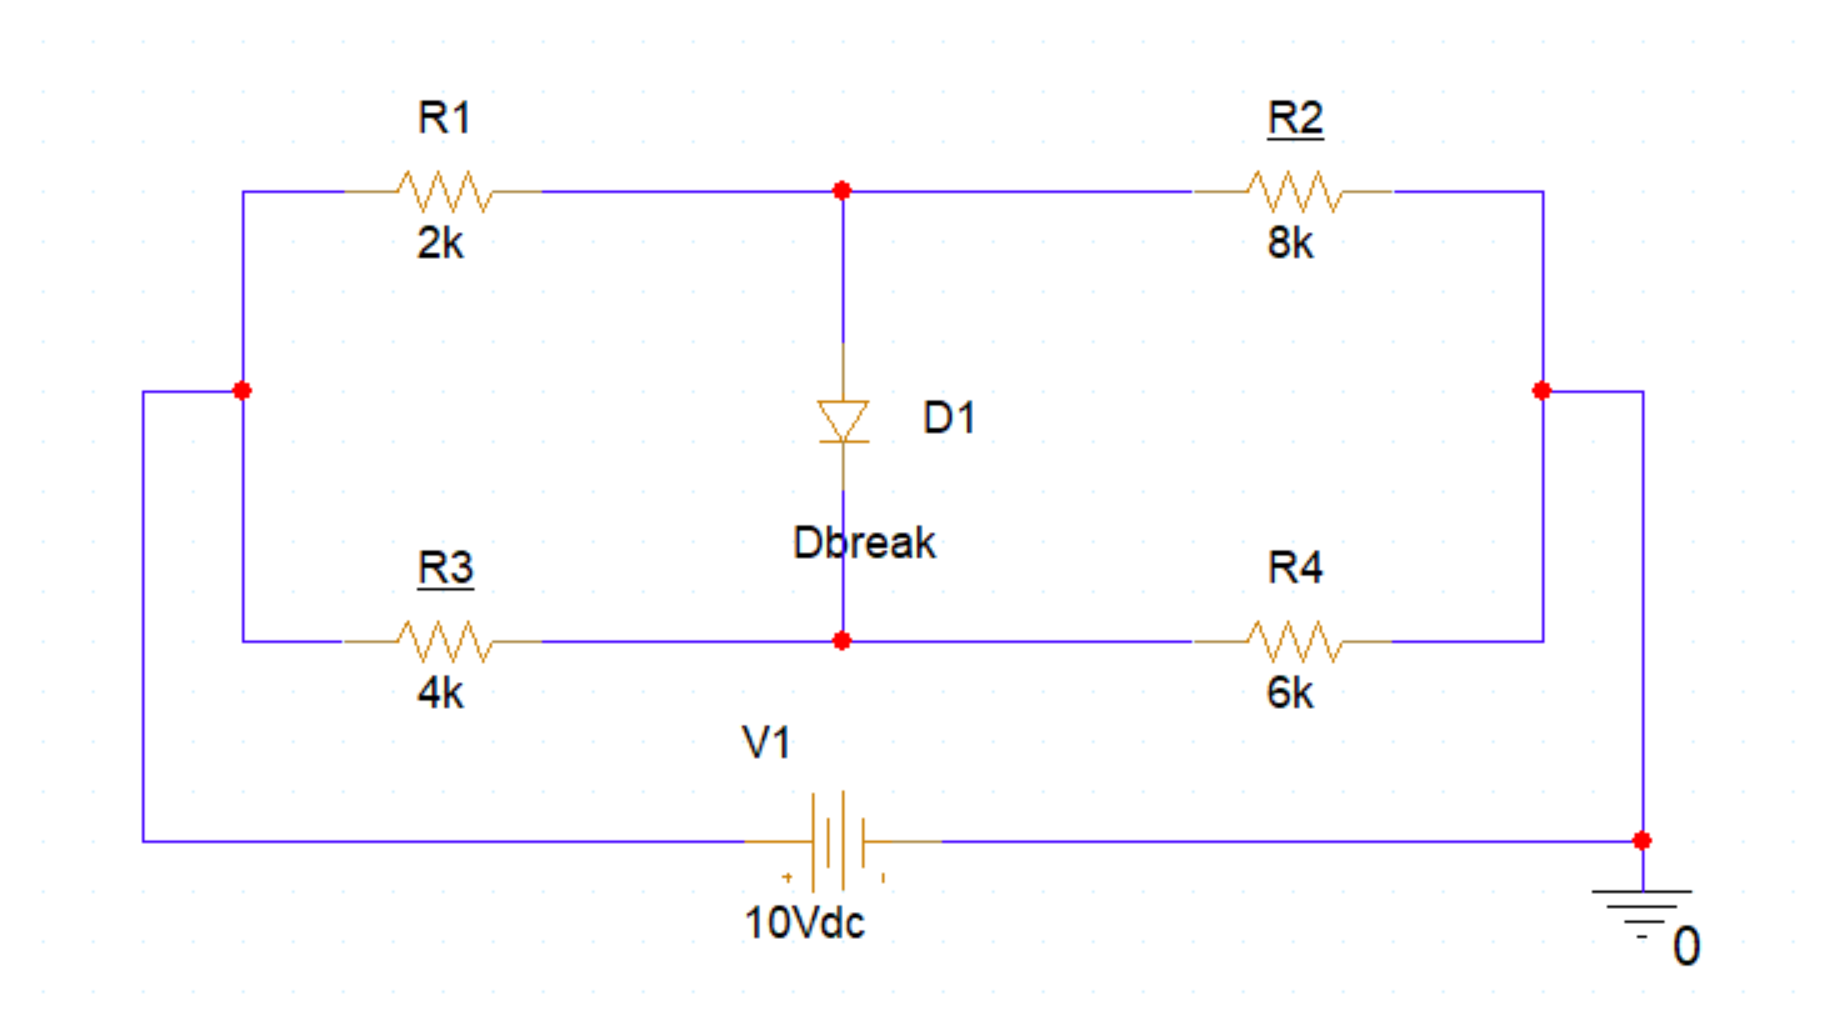
\includegraphics[scale=0.28]{graphics/ex3/f1.png}
    \caption{Phân tích mạch với diode}
\end{figure}

\subsection{Tính toán lý thuyết}
Giả sử điện áp ở cực dương và cực âm của diode V1 và V2. Nó được cho là
rằng diode đang ở chế độ phân cực thuận.

Theo chế độ diode thực tế: \(V_1 -V_2 = 0,7V\)

Học sinh được đề nghị xây dựng các phương trình để xác định dòng điện chạy qua tất cả các
điện trở.
 
\pagebreak
\textbf{Giải:}


{Ta sử dụng Kirchhoff's Vontage Law (KVL) cho 3 vòng lặp sau:

Vòng (1): \(2k.I_{R1} - 4k.I_{R3} + V_D = 0\)

Vòng (2): \(8k.I_{R2} - 6k.I_{R4} - V_D = 0\)

Vòng (3): \(4k.I_{R3} + 6k.I_{R4} - V = 0\)

Ta sử dụng Kirchhoff's Current Law (KCL) cho 3 nút sau:

Nút (A): \(I = I_{R1} + I_{R3}\) 

Nút (B): \(I_{R1} = I_D + I_{R2}\)

Nút (C): \(I_{R4} = I_D + I_{R3}\)}
\begin{figure}[h]
    \centering
    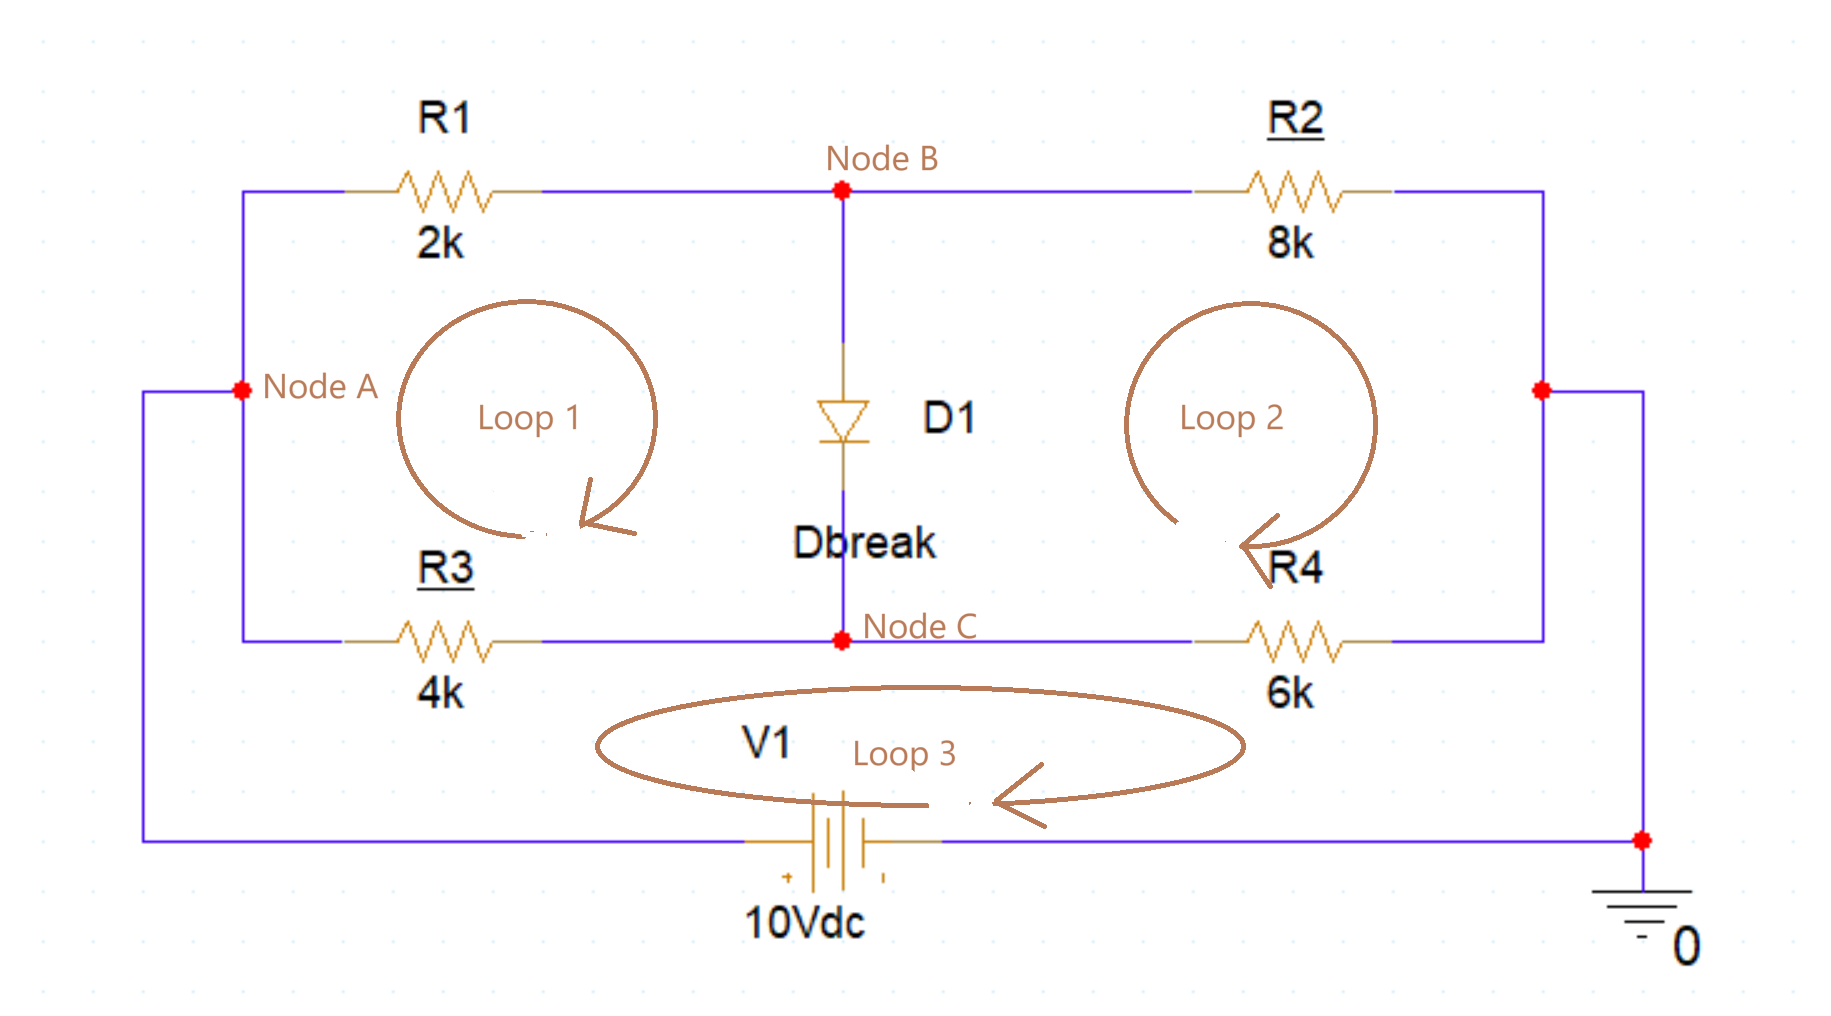
\includegraphics[scale=0.25]{graphics/ex3/f3.png}
    \caption{Minh họa}
\end{figure}

Ta có \(V_D = V_1 - V_2 = 0,7 (V)\)

\begin{align}
    \begin{cases}
    2k.I_{R1} - 4k.I_{R3} = -0,7\\
    8k.I_{R2} - 6k.I_{R4} = 0,7\\
    6k.I_{R4} + 4k.I_{R3} = V\\
    I_{R1} - I_{R2} + I_{R3} - I_{R4} = 0 \hspace*{1cm}\text{ (Lấy (B) - (C)) } 
    \end{cases}
\end{align}
\newpage
\subsection{Mô phỏng PSpice}
Cấu hình điểm thiên vị được sử dụng để chạy mô phỏng trong bài tập này. Học sinh được đề xuất
để chụp màn hình trên PSpice hiển thị dòng điện và điện áp trong mạch.
\begin{figure}[h]
    \centering
    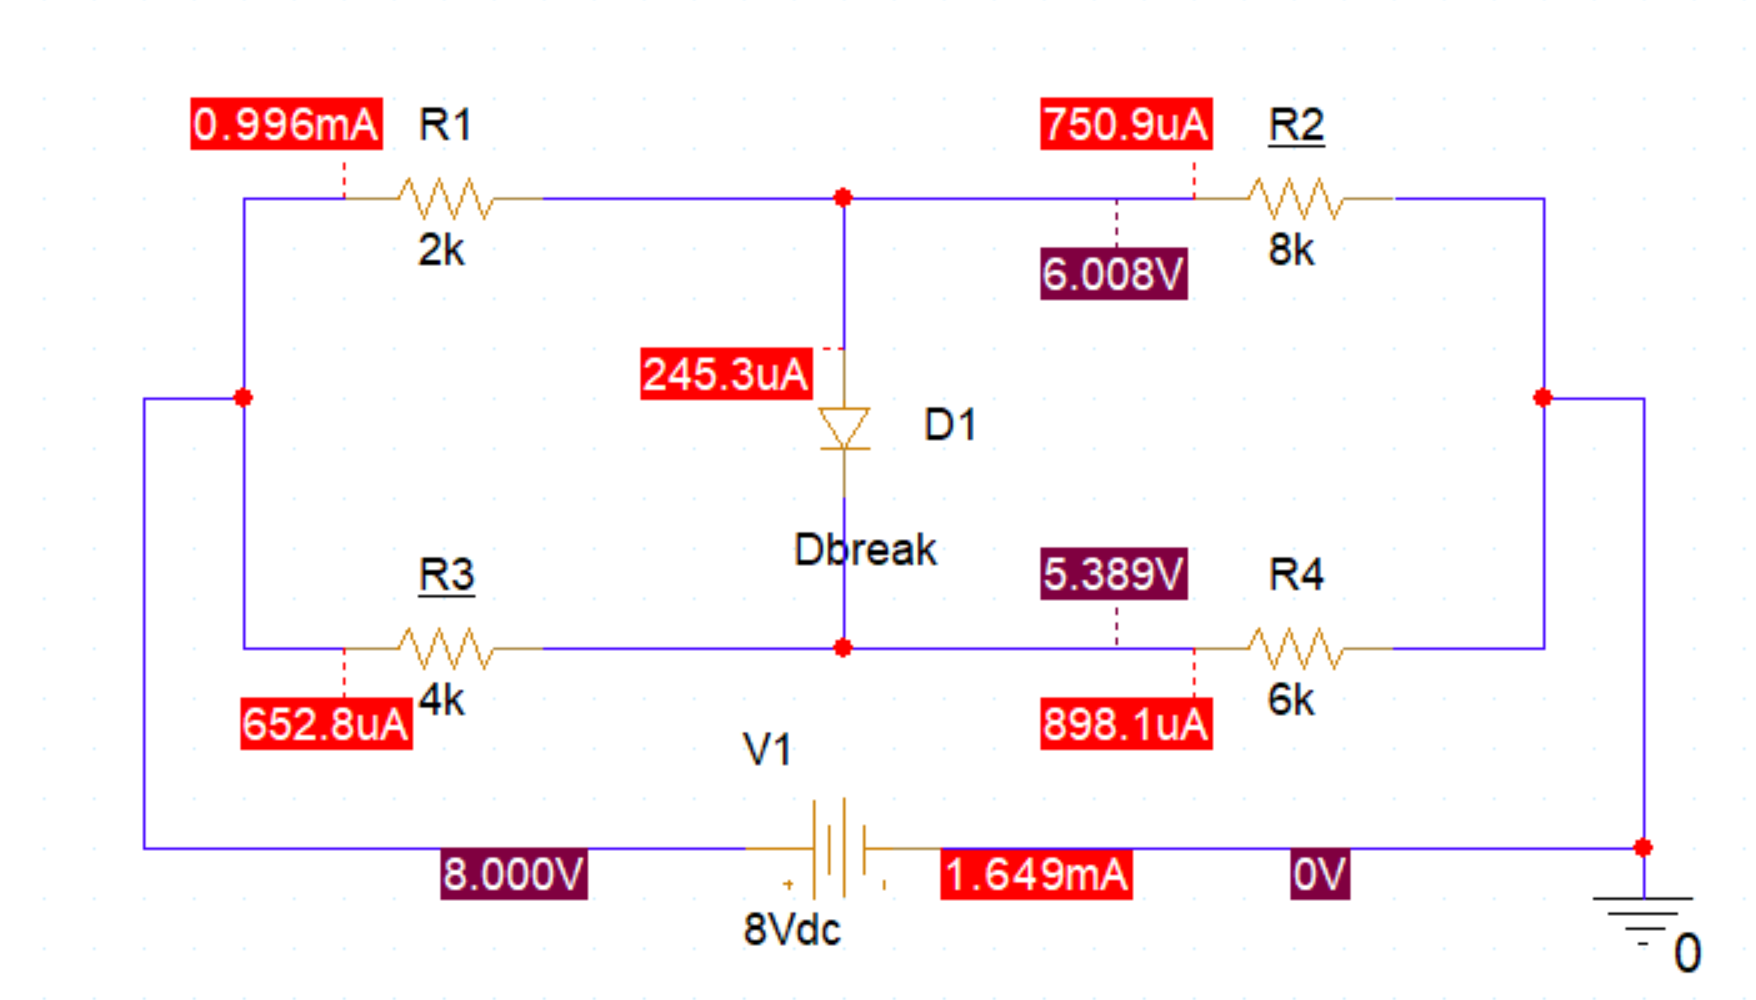
\includegraphics[scale=0.27]{graphics/ex3/f2.png}
    \caption{Mạch với V = 8V}
    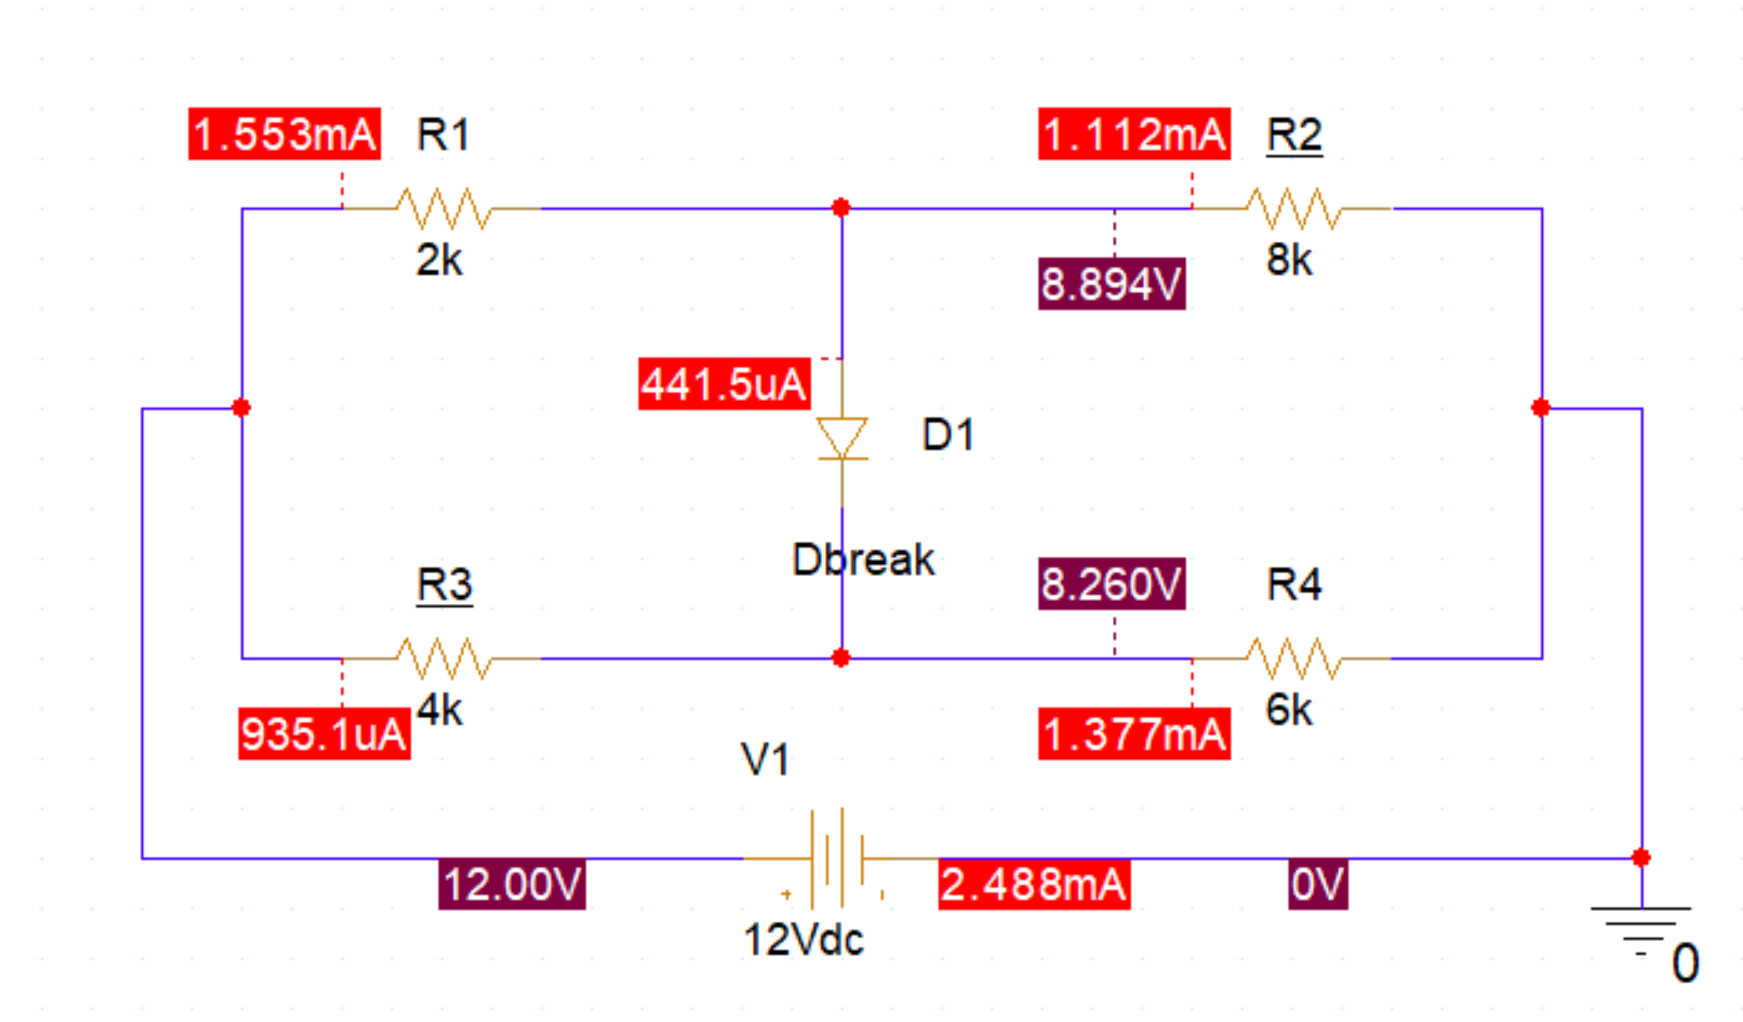
\includegraphics[scale=0.27]{graphics/ex3/f4.png}
    \caption{Mạch với V = 12V}
\end{figure}
\pagebreak
\subsection{So sánh}
Học sinh phải tóm tắt kết quả tính toán lý thuyết và PSpice
mô phỏng và điền vào bảng dưới đây.

{\scriptsize\begin{tabular}{|c|c|c|c|c|c|c|c|c|c|c|c|c|}
    \hline
     & \multicolumn{5}{c}{Theory Calculation} & & \multicolumn{5}{c}{PSpice Simulation} &\\
    \hline
    & \(I_{R1}\) & \(I_{R2}\) & \(I_{R3}\) & \(I_{R4}\) & \(V_1\) & \(V_2\) & \(I_{R1}\) & \(I_{R2}\) & \(I_{R3}\) & \(I_{R4}\) & \(V_1\) & \(V_2\)\\
    \hline
    V = 8 V & 0,980 & 0,755 & 0,665 & 0,890 & 6, 040 & 5,340 & 0,996 & 0,751 & 0,653 & 0,898 & 6,008 & 5,389\\
& (mA) & (mA) & (mA) & (mA) & (V) & (V) & (mA) & (mA) & (mA) & (mA) & (V) & (V)\\
\hline
V = 12 V & 1,54 & 1,115 & 0,945 & 1,370 & 8,92 & 8,22 & 1,553 & 1,112 & 0,935 & 1,377 & 8,894 & 8,260\\
& (mA) & (mA) & (mA) & (mA) & (V) & (V) & (mA) & (mA) & (mA) & (mA) & (V) & (V)\\
\hline
\end{tabular}}
\pagebreak
